%!TEX root = ../dissertation.tex
\begin{savequote}[75mm]
This is some random quote to start off the chapter.
\qauthor{Firstname lastname}
\end{savequote}

\chapter{Model and approach}

\todo{rivedere il titolo del capitolo}

SCALETTA:

* Visual branch
  * proposal 
  * object generator
* textual branch
  word embedding (w2v, glove)
* concept branch
* loss
* training and inference

\begin{figure}
  \centering
  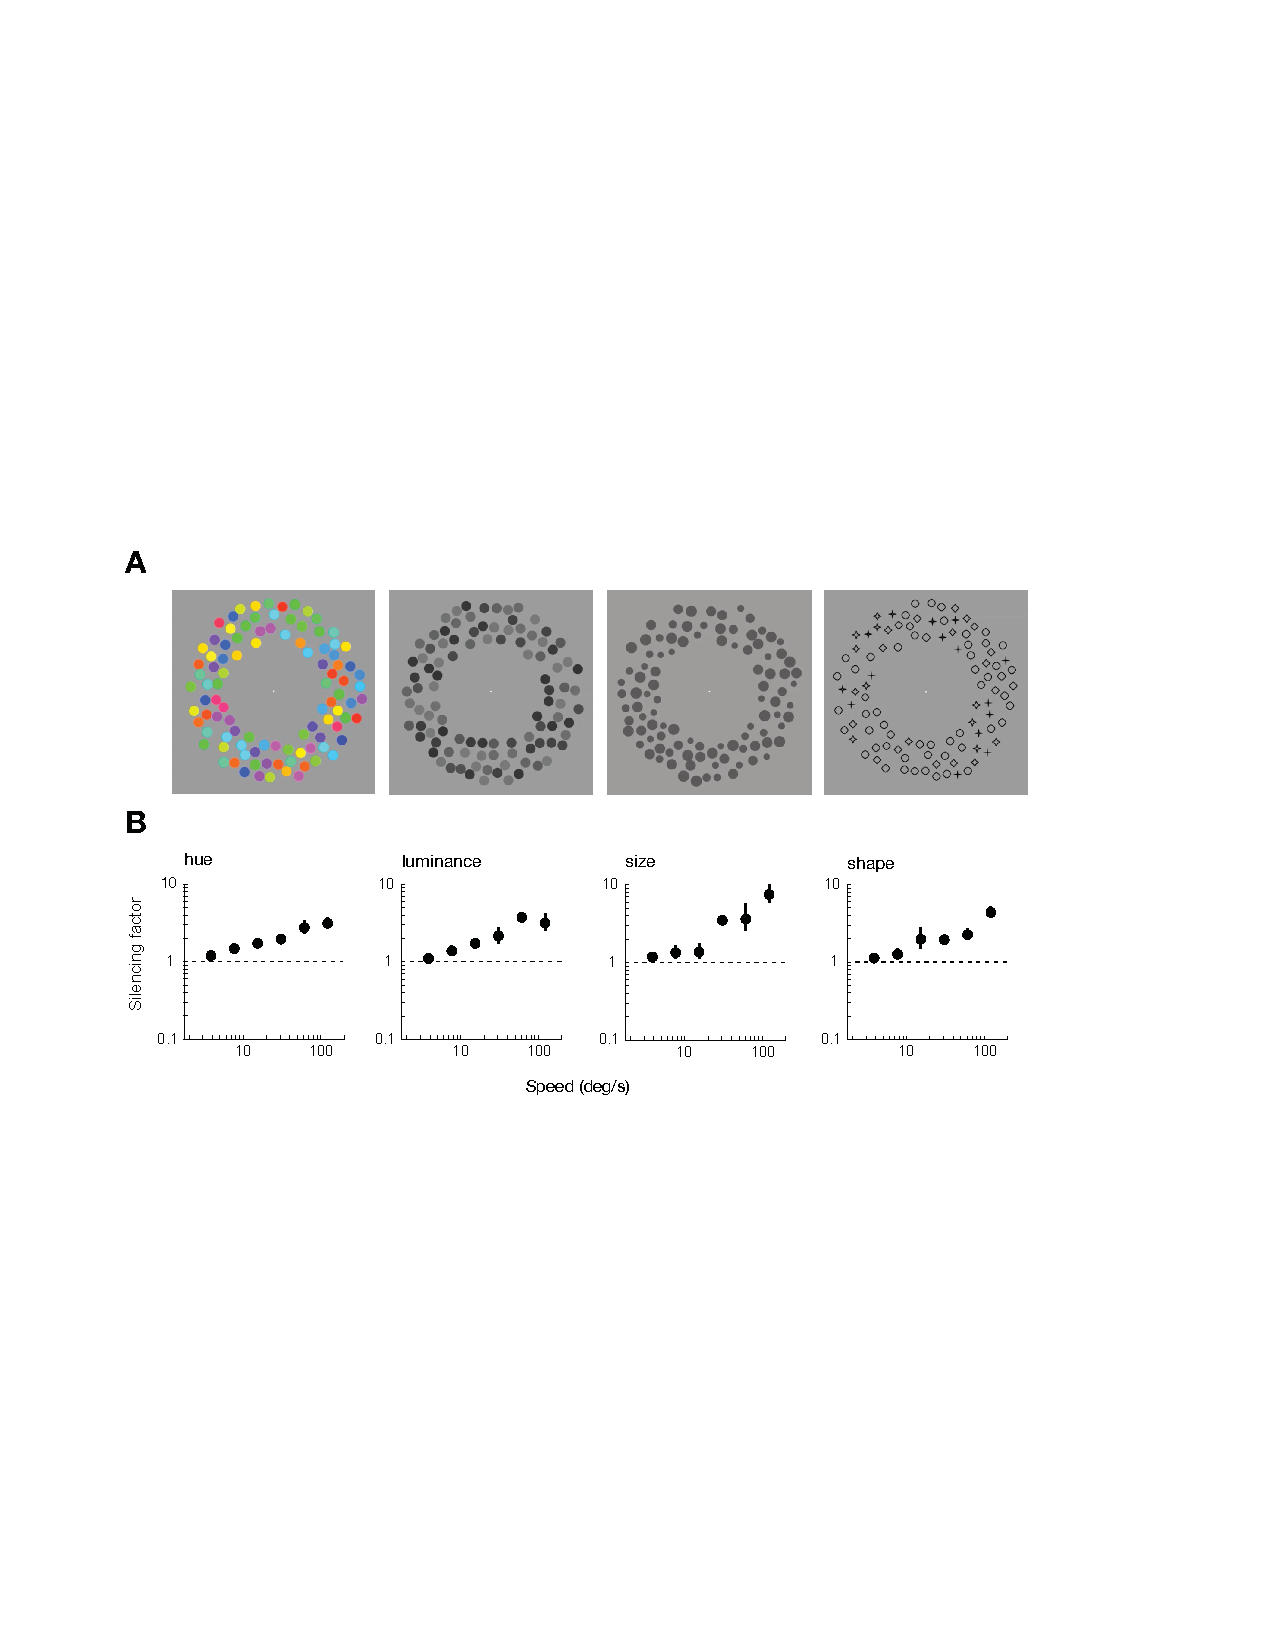
\includegraphics[width=.6\textwidth]{figures/fig1.pdf}
  \caption[TODO]{TODO: desc}
  \label{fig:model-architecture}
\end{figure}

\section{Model}

\subsection{Visual Branch}

Our model, outlined in Fig.~\ref{fig:model-architecture}, follows a
typical basic architecture for visual textual grounding tasks. It is
based on a two-stage approach in which, initially, a pre-trained
object detector (see Sec.~\ref{sec:object-detection-recognition}) is
used to extract, from a given image $\bm{I}$, a set of $k$ bounding
box proposals $\calP_{\bm{I}} = \{ \bm{p}_i \}^k_{i=1}$, where $p_i
\in \Rset^4$, jointly with features $H^v = \{ \bm{h}^v_i \}^k_{i=1}$,
where $\bm{h}^v_i \in \Rset^v$. The features represent the internal
object detector activation values before the classification layers and
regression layer for bounding boxes. Moreover, our model extracts the
spatial features $H^s = \{ \bm{h}^s_i \}^k_{i=1}$, where $\bm{h}^s_i
\in \Rset^s$ from all the bounding boxes proposals, with the spatial
features for the proposal $\bm{p}_i$ defined as:
\begin{equation}
  \bm{h}^s_i = \left[ \frac{x1}{wt}, \frac{y1}{ht}, \frac{x2}{wt}, \frac{y2}{ht}, \frac{(x2 - x1) \times (y2 - y1)}{wt \times ht}  \right]
\end{equation}
where $(x1, y1)$ refers to the top-left bounding box corner, $(x2,
y2)$ refers to the bottom-right bounding box corner, $wt$ and $ht$ are
the width and height of the image, respectively. Both visual and
spatial features are then concatenated, thus leading to a set of new
vectorial representations $H^{||} = \{ \bm{h}^{||}_{jz} \}_{j \in [1,
\ldots, m], z \in [1, \ldots, k]}$, where vectors $\bm{h}^{||}_{jz}$
are defined as:
\begin{equation}
  \bm{h}^{||}_{jz} = \Big( \bm{W}^{||} \left( \bm{h}^s_z || L1(\bm{h}^v_z) \right) + \bm{b}^{||} \Big) 
\end{equation}
where $||$ indicates the concatenation operator, $\bm{h}^{||}_{jz} \in
\Rset^c$, $\bm{W}^{||} \in \Rset^{c \times (s + v)}$ is a matrix
of weights, and $\bm{b}^{||} \in \Rset^c$ is a bias vector.

We also assume that the object detector returns, for each $\bm{p}_i$,
a probability distribution $Pr_{Cls}(\bm{p}_i)$ over a set $Cls$ of
predefined classes, i.e. the probability for each class $\zeta \in
Cls$ that the content of the bounding box $\bm{p}_i$ belongs to
$\zeta$. This information is typically returned by most of the object
detectors, and it will be used to define our novel loss function.
\todo{UPDATE: to define our...}

\subsection{Textual Branch}

Regarding the textual features extraction, given a noun phrase
$\bm{q}_j$, initially all its words $W^{\bm{q}_j} = \{ w^{\bm{q}_j}_i
\}^l_{i=1}$ are embedded in a set of vectors $E^{\bm{q}_j} =
\{e^{\bm{q}_j}_i \}^l_{i=1}$ where $e^{\bm{q}_j}_i \in \Rset^w$, where
$w$ is the size of the embedding. Then, our model applies a LSTM (see
Sec.~\ref{subsec:gated-rnn}) neural network to generate from the
sequence of word embeddings only one new embedding $\bm{h}^*_j$ for
each phrase $\bm{q}_j$. This textual features extraction is defined
as:
\begin{equation}
  \bm{h}^*_j = L1(LSTM(E^{\bm{q}_j}))
\end{equation}
where $\bm{h}^*_j \in \Rset^t$ is the LSTM output of the last word in
the noun phrase $\bm{q}_j$ , and $L1$ is the L$1$ normalization
function.
